% Options for packages loaded elsewhere
% Options for packages loaded elsewhere
\PassOptionsToPackage{unicode}{hyperref}
\PassOptionsToPackage{hyphens}{url}
\PassOptionsToPackage{dvipsnames,svgnames,x11names}{xcolor}
%
\documentclass[
  english,
  12pt,
  a4paper,
]{scrartcl}
\usepackage{xcolor}
\usepackage[top=20mm, left=25mm, right=20mm, bottom=25mm]{geometry}
\usepackage{amsmath,amssymb}
\setcounter{secnumdepth}{5}
\usepackage{iftex}
\ifPDFTeX
  \usepackage[T1]{fontenc}
  \usepackage[utf8]{inputenc}
  \usepackage{textcomp} % provide euro and other symbols
\else % if luatex or xetex
  \usepackage{unicode-math} % this also loads fontspec
  \defaultfontfeatures{Scale=MatchLowercase}
  \defaultfontfeatures[\rmfamily]{Ligatures=TeX,Scale=1}
\fi
\usepackage{lmodern}
\ifPDFTeX\else
  % xetex/luatex font selection
  \setmainfont[]{Times New Roman}
  \setsansfont[]{Times New Roman}
  \setmathfont[]{TeX Gyre Termes}
\fi
% Use upquote if available, for straight quotes in verbatim environments
\IfFileExists{upquote.sty}{\usepackage{upquote}}{}
\IfFileExists{microtype.sty}{% use microtype if available
  \usepackage[]{microtype}
  \UseMicrotypeSet[protrusion]{basicmath} % disable protrusion for tt fonts
}{}
\makeatletter
\@ifundefined{KOMAClassName}{% if non-KOMA class
  \IfFileExists{parskip.sty}{%
    \usepackage{parskip}
  }{% else
    \setlength{\parindent}{0pt}
    \setlength{\parskip}{6pt plus 2pt minus 1pt}}
}{% if KOMA class
  \KOMAoptions{parskip=half}}
\makeatother
% Make \paragraph and \subparagraph free-standing
\makeatletter
\ifx\paragraph\undefined\else
  \let\oldparagraph\paragraph
  \renewcommand{\paragraph}{
    \@ifstar
      \xxxParagraphStar
      \xxxParagraphNoStar
  }
  \newcommand{\xxxParagraphStar}[1]{\oldparagraph*{#1}\mbox{}}
  \newcommand{\xxxParagraphNoStar}[1]{\oldparagraph{#1}\mbox{}}
\fi
\ifx\subparagraph\undefined\else
  \let\oldsubparagraph\subparagraph
  \renewcommand{\subparagraph}{
    \@ifstar
      \xxxSubParagraphStar
      \xxxSubParagraphNoStar
  }
  \newcommand{\xxxSubParagraphStar}[1]{\oldsubparagraph*{#1}\mbox{}}
  \newcommand{\xxxSubParagraphNoStar}[1]{\oldsubparagraph{#1}\mbox{}}
\fi
\makeatother


\usepackage{longtable,booktabs,array}
\usepackage{calc} % for calculating minipage widths
% Correct order of tables after \paragraph or \subparagraph
\usepackage{etoolbox}
\makeatletter
\patchcmd\longtable{\par}{\if@noskipsec\mbox{}\fi\par}{}{}
\makeatother
% Allow footnotes in longtable head/foot
\IfFileExists{footnotehyper.sty}{\usepackage{footnotehyper}}{\usepackage{footnote}}
\makesavenoteenv{longtable}
\usepackage{graphicx}
\makeatletter
\newsavebox\pandoc@box
\newcommand*\pandocbounded[1]{% scales image to fit in text height/width
  \sbox\pandoc@box{#1}%
  \Gscale@div\@tempa{\textheight}{\dimexpr\ht\pandoc@box+\dp\pandoc@box\relax}%
  \Gscale@div\@tempb{\linewidth}{\wd\pandoc@box}%
  \ifdim\@tempb\p@<\@tempa\p@\let\@tempa\@tempb\fi% select the smaller of both
  \ifdim\@tempa\p@<\p@\scalebox{\@tempa}{\usebox\pandoc@box}%
  \else\usebox{\pandoc@box}%
  \fi%
}
% Set default figure placement to htbp
\def\fps@figure{htbp}
\makeatother


% definitions for citeproc citations
\NewDocumentCommand\citeproctext{}{}
\NewDocumentCommand\citeproc{mm}{%
  \begingroup\def\citeproctext{#2}\cite{#1}\endgroup}
\makeatletter
 % allow citations to break across lines
 \let\@cite@ofmt\@firstofone
 % avoid brackets around text for \cite:
 \def\@biblabel#1{}
 \def\@cite#1#2{{#1\if@tempswa , #2\fi}}
\makeatother
\newlength{\cslhangindent}
\setlength{\cslhangindent}{1.5em}
\newlength{\csllabelwidth}
\setlength{\csllabelwidth}{3em}
\newenvironment{CSLReferences}[2] % #1 hanging-indent, #2 entry-spacing
 {\begin{list}{}{%
  \setlength{\itemindent}{0pt}
  \setlength{\leftmargin}{0pt}
  \setlength{\parsep}{0pt}
  % turn on hanging indent if param 1 is 1
  \ifodd #1
   \setlength{\leftmargin}{\cslhangindent}
   \setlength{\itemindent}{-1\cslhangindent}
  \fi
  % set entry spacing
  \setlength{\itemsep}{#2\baselineskip}}}
 {\end{list}}
\usepackage{calc}
\newcommand{\CSLBlock}[1]{\hfill\break\parbox[t]{\linewidth}{\strut\ignorespaces#1\strut}}
\newcommand{\CSLLeftMargin}[1]{\parbox[t]{\csllabelwidth}{\strut#1\strut}}
\newcommand{\CSLRightInline}[1]{\parbox[t]{\linewidth - \csllabelwidth}{\strut#1\strut}}
\newcommand{\CSLIndent}[1]{\hspace{\cslhangindent}#1}

\ifLuaTeX
\usepackage[bidi=basic]{babel}
\else
\usepackage[bidi=default]{babel}
\fi
\ifPDFTeX
\else
\babelfont{rm}[]{Times New Roman}
\fi
% get rid of language-specific shorthands (see #6817):
\let\LanguageShortHands\languageshorthands
\def\languageshorthands#1{}
\ifLuaTeX
  \usepackage[english]{selnolig} % disable illegal ligatures
\fi


\setlength{\emergencystretch}{3em} % prevent overfull lines

\providecommand{\tightlist}{%
  \setlength{\itemsep}{0pt}\setlength{\parskip}{0pt}}



 


\usepackage{setspace}
\usepackage{tocloft}
\renewcommand{\cftfigpresnum}{Fig. }
\renewcommand{\cfttabpresnum}{Table }
\addtolength{\cftfignumwidth}{2em}
\addtolength{\cfttabnumwidth}{2em}
\usepackage{siunitx}
\sisetup{output-decimal-marker={.}}
\usepackage[noblocks]{authblk}
\renewcommand*{\Authsep}{, }
\renewcommand*{\Authand}{, }
\renewcommand*{\Authands}{, }
\renewcommand\Affilfont{\small}
\makeatletter
\@ifpackageloaded{caption}{}{\usepackage{caption}}
\AtBeginDocument{%
\ifdefined\contentsname
  \renewcommand*\contentsname{Table of contents}
\else
  \newcommand\contentsname{Table of contents}
\fi
\ifdefined\listfigurename
  \renewcommand*\listfigurename{List of Figures}
\else
  \newcommand\listfigurename{List of Figures}
\fi
\ifdefined\listtablename
  \renewcommand*\listtablename{List of Tables}
\else
  \newcommand\listtablename{List of Tables}
\fi
\ifdefined\figurename
  \renewcommand*\figurename{Figure}
\else
  \newcommand\figurename{Figure}
\fi
\ifdefined\tablename
  \renewcommand*\tablename{Table}
\else
  \newcommand\tablename{Table}
\fi
}
\@ifpackageloaded{float}{}{\usepackage{float}}
\floatstyle{ruled}
\@ifundefined{c@chapter}{\newfloat{codelisting}{h}{lop}}{\newfloat{codelisting}{h}{lop}[chapter]}
\floatname{codelisting}{Listing}
\newcommand*\listoflistings{\listof{codelisting}{List of Listings}}
\makeatother
\makeatletter
\makeatother
\makeatletter
\@ifpackageloaded{caption}{}{\usepackage{caption}}
\@ifpackageloaded{subcaption}{}{\usepackage{subcaption}}
\makeatother
\usepackage{bookmark}
\IfFileExists{xurl.sty}{\usepackage{xurl}}{} % add URL line breaks if available
\urlstyle{same}
\hypersetup{
  pdftitle={A quantitative assessment of expert-rated Smart City Development on quality of life in the United States},
  pdfauthor={Nicholas Victor Julius Alexander; Emilia TITAN; Claudiu HERTELIU},
  pdflang={en},
  colorlinks=true,
  linkcolor={black},
  filecolor={Maroon},
  citecolor={black},
  urlcolor={black},
  pdfcreator={LaTeX via pandoc}}


\title{A quantitative assessment of expert-rated Smart City Development
on quality of life in the United States}


\author[1]{Nicholas Victor Julius Alexander}
\author[1]{Emilia TITAN}
\author[1]{Claudiu HERTELIU}

\affil[1]{Department of Statistics and Econometrics, Bucharest
University for Economic Studies}


\date{Last Updated on April 28, 2025, 03:38 UTC}
\begin{document}
\maketitle


Smart City Development (SCD) is one of the most prevalent paradigms in
urban planning in the developed world, emerging as a response to
post-industrial demographic transformations. In developed countries,
including the United States (US), urban population declined from the
1930s until the 1990s, owing to the demographic decline of populations
born in these cities and the loss of many jobs requiring physical
presence in urban areas. But, unexpectedly, the Shrinking Cities
transformation stopped about three decades ago and first-world urban
populations are once again increasing (Baudet-Michel and Paulus
(\citeproc{ref-Baudet-MichelChapitredecroissanceurbaine2021}{2021});
Frey (\citeproc{ref-FreyNewcensusdata2024}{2024}); Ministerio de
Transportes, Movilidad y Agenda Urbana, DG de Vivienda y Suelo
(\citeproc{ref-MinisteriodeTransportesMovilidadyAgendaUrbanaDGdeViviendaySueloAreasurbanasEspana2022}{2022});
National Records of Scotland Web Team
(\citeproc{ref-NationalRecordsofScotlandWebTeamPopulationGrowsLarge2021}{2021})).
On the other hand, in developing countries, there are large demographic
shifts from rural to urban environments, replicating the earlier
population flow experienced by the developed world in the early 20th
century (United Nations, Department of Economic and Social Affairs,
Population Division
(\citeproc{ref-UnitedNationsDepartmentofEconomicandSocialAffairsPopulationDivisionWorldCities20182018}{2018})).

There is concern that an increase in urban densities could lead to a
loss of quality of life (QoL), as witnessed in the West in the early
20th century. Despite significant changes in city zoning and building
codes, recent cross-sectional observational studies indicate an inverse
correlation between subjective well-being and population density in US
cities (Winters and Li
(\citeproc{ref-WintersUrbanisationnaturalamenities2016}{2016})). On the
other hand, similar studies conducted in Western Europe (Mouratidis
(\citeproc{ref-MouratidisCompactcityurban2019}{2019})) or focused on
specific age cohorts (Okulicz-Kozaryn and Valente
(\citeproc{ref-Okulicz-KozarynNourbanmalaise2019}{2019})) suggest that
this inverse correlation is not universally present. Several attempts to
explain this discrepancy start assume the inclusion of Type II
statistical errors, or epoch-specific idiosyncrasies within each sample.
A third hypothesis attributes the difference between American and
European density - QoL relationship to cultural differences, as captured
by the witticism ``Americans live to work, while Europeans work to
live.'' (Okulicz-Kozaryn
(\citeproc{ref-Okulicz-KozarynEuropeansworklive2011}{2011})) This
approach suggests that culture-specific social structures facilitate
Europeans' higher tolerance for increased demographic density. A
relevant implication would be that policies allowing Americans to live
similarly to Western Europeans could improve the formers' perception of
high urban density.

SCD can be seen as a practical application of this corollary. Experts
from both sides of the Atlantic believe that cities with shorter
distances between key locations, public spaces facilitating social
interactions, accessible public transport, and green spaces tend to
provide a better QoL at the same objective level of demographic density,
compared to cities developed around the personal automobile or gated
communities. Furthermore, they argue that an active effort to reshape
cities from an individualistic to a more community-focused model would
enhance urban residents' QoL (Caragliu, Bo, and Nijkamp
(\citeproc{ref-CaragliuSmartcitiesEurope2011}{2011}); Nivola
(\citeproc{ref-NivolaAreEuropescities1999}{1999})). This trend toward
community-oriented urban development is generally linked to the belief
that the introduction of novel technologies, such as real-time
monitoring, may counter potential urban decline. Within this framework,
the European Commission (EC) has defined the smart city as ``a place
where traditional networks and services are made more efficient with the
use of digital solutions for the benefit of its inhabitants and
business.'' (European Commission
(\citeproc{ref-EuropeanCommissionSmartcities2016}{2016})) Among the
goals set by the EC for developing smart cities are the efficient use of
local resources, pollution minimization, improved availability of public
transportation, safe drinking water and sanitation infrastructure,
energy-efficient lighting and heating, and streamlined citizen-authority
interactions. In short, the European understanding of SCD stresses QoL
improvement.

By contrast, in the US, the National Institute of Standards and
Technology (NIST) defines SCD as ``the effective use of digital
technologies to deliver prioritized services and benefits to achieve
community goals.'' (Serrano et al.
(\citeproc{ref-SerranoSmartcitiescommunities2022}{2022})) In addition to
improved services, NIST criteria for a smart city include the alignment
of metrics and budget priorities with citizens preferences, investment
optimization, and rich information streams. While these gauges can be
useful in evaluating cities or city governments' efforts, the
cost-effective structure of NIST's goals is notable. It is indeed
intuitive that SCD evaluation should include a metric of public
investment efficiency, but it is unclear how this efficiency can be
measured in a smart way. For example, it is unclear whether an urban
highway is a smart amenity. A highway is superior in terms of speed to a
bicycle lane, but, at the same time, urban highways degrades the
well-being of the supposed beneficiaries, to the point that, even in the
US, housing near the highway is sold at a discount (Samuels and Freemark
(\citeproc{ref-Samuelspollutedlifehighway2022}{2022})). According to the
NIST definition, US urban planners were the first in the world to apply
intelligent city management techniques, in 1970, when they used aerial
photographs to assess the quality of Los Angeles' housing stock
(Stübinger and Schneider
(\citeproc{ref-StubingerUnderstandingSmartCity2020}{2020})). Again, it
is not immediately obvious how this approach improved the quality of
life of the residents of the city surveyed in this hi-tech manner.
Arguably, in the US understanding of the term ``smart city'', the
purpose is subordinated to the process.

Between the concept of the smart city as defined by the EC and the one
defined by the NIST, there exists a broad spectrum of definitions,
ranging from those centered on QoL to those focused on the novelty of
development methods. According to a recent European review (Bolívar
(\citeproc{ref-BolivarsearchSmartSource2019}{2019})), the various
definitions encompass, with varying emphasis, ``smart economy, smart
people, smart governance, smart mobility, smart environment, and smart
living''. Unfortunately, almost all the articles cited in this review
offer definitions without applying them to concrete data, and,
therefore, without quantive scaling for any of the criteria. Such an
approach makes it impossible to compare cities based on SCD indices, or
even to appreciate dynamics within the same city. We are aware of only
one study that provides quantitative evidence supporting the correlation
between QoL and a numeric composite metric of SCD using the previously
mentioned six domains (Wang and Zhou
(\citeproc{ref-WangDoessmartcity2023}{2023})), but it is limited to
China. A quantitative assessment of SCD in the US and the EU is urgently
needed, given that its theoretical foundation - the hypothesis that a
communal way of life is superior to an individualistic one in terms of
QoL - appears accepted solely on axiomatic grounds, and yet it guides
the development of several first-order urban centers (New York and
Vienna, among others reviewed in Choi and Caicedo
(\citeproc{ref-Choicomparativeanalysisseven2023}{2023})).

In this study, we analyze quantitatively the correlation between the SCD
and QoL. SCD metrics were obtained from two European academic centers,
the International Institute for Management Development (IMD) in Lausanne
and the Instituto de Estudios Superiores de la Empresa (IESE) in
Barcelona. Both institutions host expert groups, who publish periodic
world SCD city rankings, based on published, well-defined SCD criteria.
Additionally, both sets of rankings include domain metrics, allowing
identification of stronger and weaker SCD domains in the assessed
cities. For general QoL rankings, we use, as a starting point, the
scores from the well-known US News \& World (USNW) report ranking US
cities, based on quantitative and survey data. For a deeper
understanding of QoL components, we use the publicly-available data from
Numbeo.com, an online platform where anonymous resident ratings and
several well-published indicators are combined, through specified
formulas, into domain indices. The analysis was limited to US cities,
primarily because a narower geographic focus reduces potential cultural
confounders, such as language differences in questionnaires and
intercultural axiological differences.

\section{Research hypotheses}\label{research-hypotheses}

H1. SCD metrics from IESE and IMD have a strong degree of correlation,
indicating that they measure similar concepts.

H2. SCD metrics from the same group of experts are correlated over time,
indicating that local authorities show a persistent interest (or lack of
interest) in SCD.

H3. Domain SCD metrics for a city are largely correlated, indicating
that local authorities pursue systemic rather than domain-specific
improvements.

H4. QoL metrics from USNW and Number.com have a strong degree of
correlation, indicating that they measure similar concepts.

H5. QoL metrics and SCD metrics correlate in cross-sectional analysis,
demonstrating an effect of SCD-oriented policies on QoL in US cities.

H6. The correlation between QoL metrics and SCD metrics is
domain-specific, with certain SCD domains (for example, smart
transportation) showing stronger associations with QoL than others.

H7. The correlation between QoL metrics and SCD metrics is
domain-specific, with certain SCD domains (for example, leisure time)
showing stronger associations with QoL than others.

\section{Data acquisition and
processing}\label{data-acquisition-and-processing}

Ten US cities were evaluated in the most recent wave of the IMD Smart
Cities Index, in 2023 (Bris et al.
(\citeproc{ref-BrisIMDSmartCity2023}{2023})). The IMD data include an
estimate of the Human Development Index (HDI) at city level, a survey on
the top five Concerns of the resident population, and a survey on the
Structures and Technologies supporting SCD. The latter assesses five
domains: governance, health and safety, mobility, professional
development opportunities, and leisure activities (copied from Bris et
al. (\citeproc{ref-BrisIMDSmartCity2023}{2023}) in Supplemental Table
1). Although the IMD report provides rankings and score from past years,
the IMD methodology has changed repeatedly and significantly, making
time series analysis less reliable. The number of respondents is not
specified, but it is stated to be representative. IMD data were
semi-automatically transcribed from the document available at imd.org.

The SCD indicators obtained from IESE include solely a score (Cities in
Motion Index, CIMI) and rankings based on that score. However,
correlation between IESE scores with IMD scores would be supportive for
the notion of a relative agreement among experts, with regards to SCD
metrics. Moreover, IESE criteria have been rather invariable, making
IESE rankings useful in evaluation of eventual chronologic trends with
regards to expert-generated SCD rankings. In 2024, the IESE criteria
covered nine domains, namely human capital, social cohesion, economy,
governance, environment, mobility, international profile, urban
planning, and technology (copied from Berrone et al.
(\citeproc{ref-BerroneIESECitiesMotion2024}{2024}) in Supplemental Table
2). The IESE overall rankings and scores data were transcribed
semi-automatically from documents published at iese.edu, and cover 8 US
cities assessed in IESE Cities in Motion 2014 (Berrone et al.
(\citeproc{ref-BerroneIESECitiesMotion2014}{2014})), as well as 19 US
cities in IESE Cities in Motion 2024 (Berrone et al.
(\citeproc{ref-BerroneIESECitiesMotion2024}{2024})).

For QoL, we used USNW rankings, compiled by experts for over fifty years
and highly influential in shaping American public perception (Bloom
(\citeproc{ref-Bloom25Citiesbest2024}{2024})). In the Best Places to
Live 2023-2024 rankings, QoL scores comprise 36\% of the overal
desirability score of a city. QoL scores are computed from metrics of
subjective well-being, crime rates, education quality, commute quality,
environment quality, and quality of healthcare services, with weights
derived from US surveys (copied from {``How We Rank the {Best Places to
Live and Retire}''} (\citeproc{ref-Howwerank2024}{n.d.}) in Supplemental
Table 3). USNW does not publish domain-specific QoL metrics. The overall
QoL score was manually extracted from the Best Places to Live and Retire
2023 ranking ({``Best {Places to Live} for Quality of Life, Ranked''}
(\citeproc{ref-BestPlacesLive2023}{2023})), available at usnews.com.

Since 2009, Numbeo.com has hosted a web platform where self-selected,
anonymous users, authenticating with their email address, may rate
cities acrss the world, based on criteria such as cost of living, cost
of housing as a proportion of income, safety, healthcare services,
climate, pollution, and commute burden. Although there are concerns
regarding data quality, as with any internet-based survey, each of the
studied cities has over 200 reviews, which reduces the impact of
malicious responses. Moreover, in addition to survey data, Numbeo also
incorporates a few official public data in the calculation of its
composite indices (detailed, based on, in Supplemental Table 4). Numbeo
is considered the best available source, especially for local prices, by
major media outlets such as The Economist (L.S.
(\citeproc{ref-LStaletwoecosystems2013}{2013})), Forbes (Barrett
(\citeproc{ref-BarrettInvestigateYouExpatriate2010}{2010})), and The New
York Times (Kugel (\citeproc{ref-KugelThingsYouCan2016}{2016})). We
manually collected overall QoL scores, as well as scores for its eight
dimensions, from numbeo.com, as displayed in April 2024.

Manually-loaded data was pasted in LibreOffice Calc 25.2.2, and the
resulting raw spreadsheet has been shared at
https://github.com/nvalexander/smartcities. Subsequently, data was
imported in VSCode 1.99.3, processed and analyzed with R 4.2.2 (R Core
Team
(\citeproc{ref-RCoreTeamlanguageenvironmentstatistical2021}{2021})), and
typeset with Quarto 1.7.29. Data wrangling and visualization relied on
the tidyverse R library, version 2.0.0 (Wickham et al.
(\citeproc{ref-tidyverse2019}{2019})). Analysis used R libraries
including tseries version 0.10.58, irr version version 0.84.1, car
version 3.1.3, broom version 1.0.8 and lmtest version 0.9.40.

Although USNW and Numbeo.com provide QoL ratings for hundreds and,
respectively thousands of US cities, the number of cities ranked by IESE
and IMD is typically around 100 across the world. For the most part we
analyzed data for all the 19 US cities featured the IESE 2024 rankings,
but only 4 US cities (New York, Los Angeles, Chivago and Philadelphia)
were assessed in all three reports used for this study. A set of 76
variables were obtained, including 59 metrics of SDC from IMD, 4 SCD
metrics from IESE, 9 QoL metrics from Numbeo.com, one QoL metrics from
USNW, and two control variables (overall USNW score and rank).

Among the 75 relevant variables 40\% of the data was missing.
Missingness ranged from 12 variables with fewer than 10\% missing data
to 3 varaibles from IEsE 2014 with more than 50\% missingness. The
overall mean skewness was low (mean absolute skewness 0.08), suggesting
limited departure from normality. Within the SCD-related variable set,
17.2\% of pairs had an absolute Pearson correlation greater than 0.7,
suggestign some redundancy among predictors. Among QoL-related
variables, 2.2\% of pairs exceeded this threshold, indicating minimal
multicollinearity.

\section{Results}\label{results}

\subsection{IESE and IMD rankings evaluate similar
constructs}\label{iese-and-imd-rankings-evaluate-similar-constructs}

Normality of the IESE 2024 and IMD 2023 ranks was assessed using
Shapiro-Wilk tests, which indicated no significant deviation from
normality (p = 0.161 and p = 0.664, respectively). The IESE composite
score, however, showed significant non-normality (p = 1.09e-04).
Accordingly, Pearson correlation was used to assess the association
between IESE and IMD rankings. The positive correlation was strong (r =
0.73, p = 0.016, df = 17).

\begin{figure}[H]

{\centering \pandocbounded{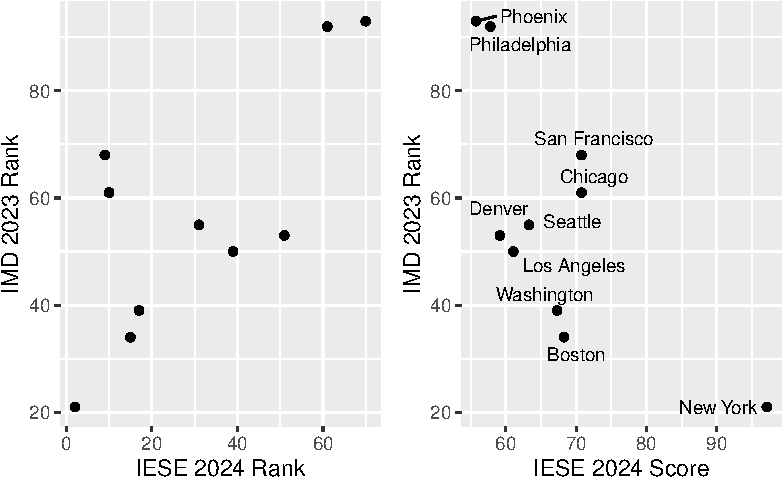
\includegraphics[keepaspectratio]{smartcities_files/figure-pdf/imdvsiese-1.pdf}}

}

\caption{Scatterplots illustrating the correlation between IMD 2023
rankings and IESE 2024 indicators.}

\end{figure}%

Figure 1 illustrates the non-normality of IESE CIMI scores, introduced
by the much higher score attributed to New York. Given the non-normality
of the IESE composite score, Spearman's rho was used to assess its
association with the IMD ranking. The rank-based correlation was -0.53
(p = 0.123, df = 17). Although the latter test was not statistically
significant, the former test indicates that IESE and IMD rankings
capture broadly similar dimensions.

\subsection{Expert SCD ratings are stable in
time}\label{expert-scd-ratings-are-stable-in-time}

Pairwise Pearson correlation analysis between consecutive IMD reports
indicate stability of IMD rankings over time. The correlation between
2019 and 2020 was high (r = 0.78, p = 0.013), as was the correlation
between 2020 and 2021 (r = 0.97, p = 3.04e-06), and between 2021 and
2023 (r = 0.97, 5.74e-06). To summarize the overall consistency across
years, we computed the intraclass correlation coefficient (ICC), using a
one-way random-effects model. The ICC was 0.77, significantly greater
than zero (F(8, 27) = 14, p = 8.18e-08), with a 95\% confidence interval
ranging from 0.51 to 0.93. These results suggest a strong persistence of
relative city rankings across the observed period.

\begin{figure}[H]

{\centering \pandocbounded{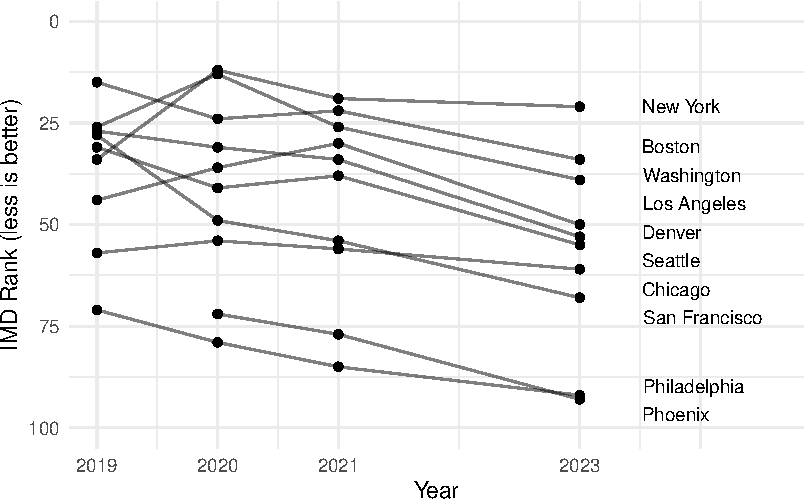
\includegraphics[keepaspectratio]{smartcities_files/figure-pdf/imdintime-1.pdf}}

}

\caption{Trajectories of IMD Smart City rankings for each city
(2019--2023)}

\end{figure}%

In addition to the statistical analysis, a plot of IMD ranks across the
four timepoints (Fig. 2) supports the notion of stable rankings, with
the general decreasing tend explained by the addition of non-US cities
that rank extremely well by IMD metrics (Canberra, Wellington,
Reykjavik, Lausanne), in a manner that does not affect the US
hierarachy.

\subsection{SCD ratings components correlate moderate between domains,
with the exception of reported
Concerns}\label{scd-ratings-components-correlate-moderate-between-domains-with-the-exception-of-reported-concerns}

Surprisingly, in the IMD survey, which provides domain metrics, not all
of the four components of the SCD assessement correlate well between
cities. Specifically, Pearson correlation analysis did not support a
correlation between HDI and the sum of IMD Technologies indicators (r =
0.27, p = 0.455). In contrast, the correlation between HDI and the sum
of IMD Structures indicators was r = 0.62, p = 0.058. The correlation
between IMD Technologies and IMD Structures was r = 0.61, p = 0.063.

The IMD Concerns sum significantly from normality (p = 0.018), unlike
the other three IMD domains. Therefore, for associations involving the
non-normally distributed IMD Concerns sum, Spearman correlations were
used instead. Evidence of a correlation between HDI and IMD Concerns was
found using Spearman's method (ρ = -0.71, p = 0.02). On the other hand,
there was no evidence for an association between Technologies and
Concerns (ρ = -0.46, p = 0.184), nor for the association between
Structures and Concerns (ρ = -0.57, p = 0.083).

A plot of these potential correlation (Fig. 3) indicates confirms that
IMD Concerns scores are not normally distributed, with an extremely low
sum of Concerns indicators for Denver. Nevertheless, Denver's exclusion
fails to improve statistical significance between the sum of IMD
Concerns indicators and the other domain indicator sums (data not
shown).

\begin{figure}[H]

{\centering \pandocbounded{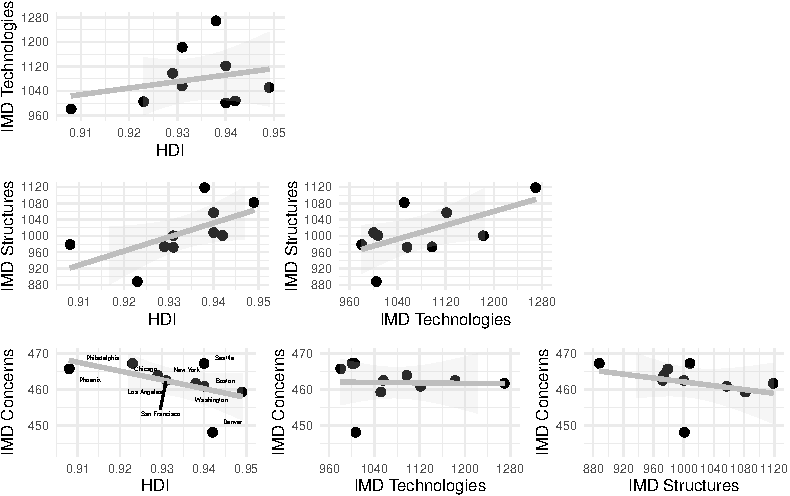
\includegraphics[keepaspectratio]{smartcities_files/figure-pdf/imdcomponentsplot-1.pdf}}

}

\caption{Correlations between IMD Smart City score domains}

\end{figure}%

\subsection{QoL metrics do not fall into
agreement}\label{qol-metrics-do-not-fall-into-agreement}

Another failure to support one of hypothese was noted when testing
Pearson correlation between the USNW and Numbeo.com QoL metrics. In the
global analysis, there was no statistical significance for an eventual
correlation (r = 0.12, p = 0.614). To explore potential partial
overlaps, Pearson correlation analysis was applied to all the possible
combinations between the USNW QoL score and each of the eight Numbeo
component indices. The only meaningful correaltion was the negative
correlation between the USNW QoL score and Numbeo Pollution Index (r =
-0.56, p = 0.014). Counterintutively, the USNW QoL score exhibited
significant positive correlation with the Numbeo Cost of Living Index (r
= 0.53, p = 0.021) and weak positive correlation with the Property Price
to Income Ratio (r = 0.46, p = 0.05). No other Numbeo components
displayed strong or statistically significant associations with the USNW
QoL score. These results, as well as the corespnding graphic
representation (Fig. 4) suggest that, while some aspects of local
affordability and environmental quality relate to the USNW metric,
broader alignment between the two systems remains limited.

\begin{figure}[H]

{\centering \pandocbounded{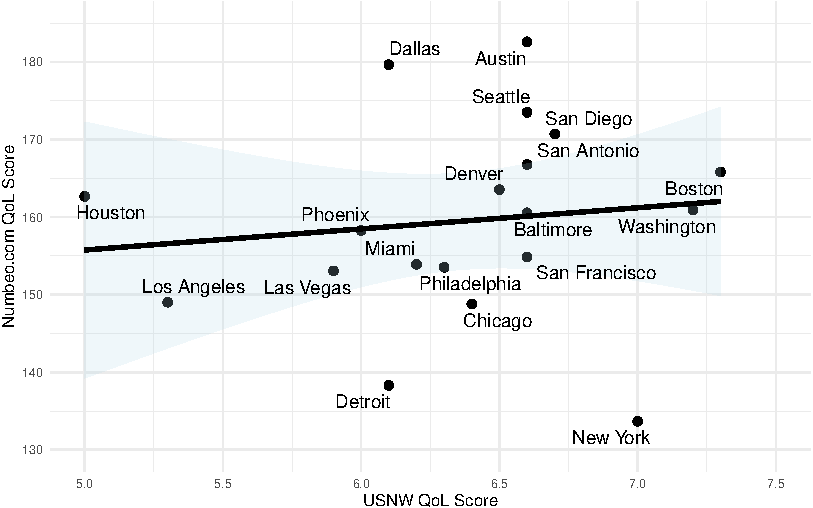
\includegraphics[keepaspectratio]{smartcities_files/figure-pdf/usnwvsnumbeoplot-1.pdf}}

}

\caption{Weak correlation between USNW and Numbeo QoL scores}

\end{figure}%

\subsection{Data does not support a correlation between SCD metrics and
QoL
metrics}\label{data-does-not-support-a-correlation-between-scd-metrics-and-qol-metrics}

The normality of the main QoL and SCD indicators was assessed using
Shapiro-Wilk tests. None of the tests rejected the null hypothesis of
normality (data not shown), justifying the use of Pearson correlation
for subsequent analyses. The correlation between USNW QoL scores and the
IMD 2023 SCD ranking was moderate and negative (r = -0.53, p = 0.118),
but did not reach statistical significance. A similar negative trend was
observed between USNW QoL scores and the IESE 2024 ranking (r = -0.43, p
= 0.068). In contrast, correlations between the Numbeo QoL score and
either SCD ranking were weak (r = 0.19 and r = 0.1, respectively) and
nonsignificant (p = 0.608 and p = 0.687, respectively).

\begin{figure}[H]

{\centering \pandocbounded{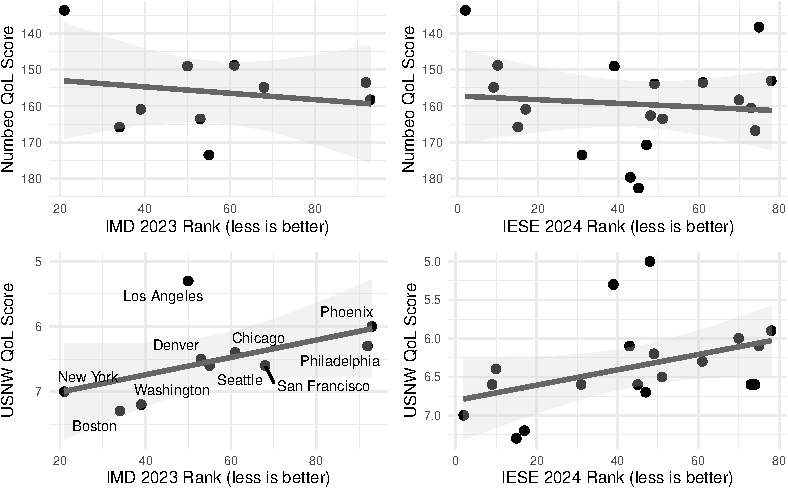
\includegraphics[keepaspectratio]{smartcities_files/figure-pdf/qolscdplot-1.pdf}}

}

\caption{Weak associations between SCD ranks and QoL scores. Rank axes
are inverted.}

\end{figure}%

A plot of the above-analyzed correlation (Fig. 5) confirms the
hypothesized trend towards better QoL rankings for cities with stronger
SCD polices, when the QoL is assessed by USNW. Paradoxically, the minute
effect that SCD policies appear to have on Numbeo.com rankings manifest
as trends towards positive correlation, that is, stronger SCD policies
associate with worse QoL Numbeo.com rankings. In the next section, we
will investigate which dimensions of Numbeo.com or IMD composite scores
are best associated with the marginal effects uncovered here.

\subsection{Numbeo.com QoL metrics are negatively correlated with most
technology-related SCD
items}\label{numbeo.com-qol-metrics-are-negatively-correlated-with-most-technology-related-scd-items}

We have seen that IMD-assessed SCD exhibit a trend towards association
with better QoL rankings, when originating from USNW. In this section,
we attempt to uncover which of the IMD domains coordinates best with
improved QoL. The general trands are illustrated in Fig. 6.

\begin{figure}[H]

{\centering \pandocbounded{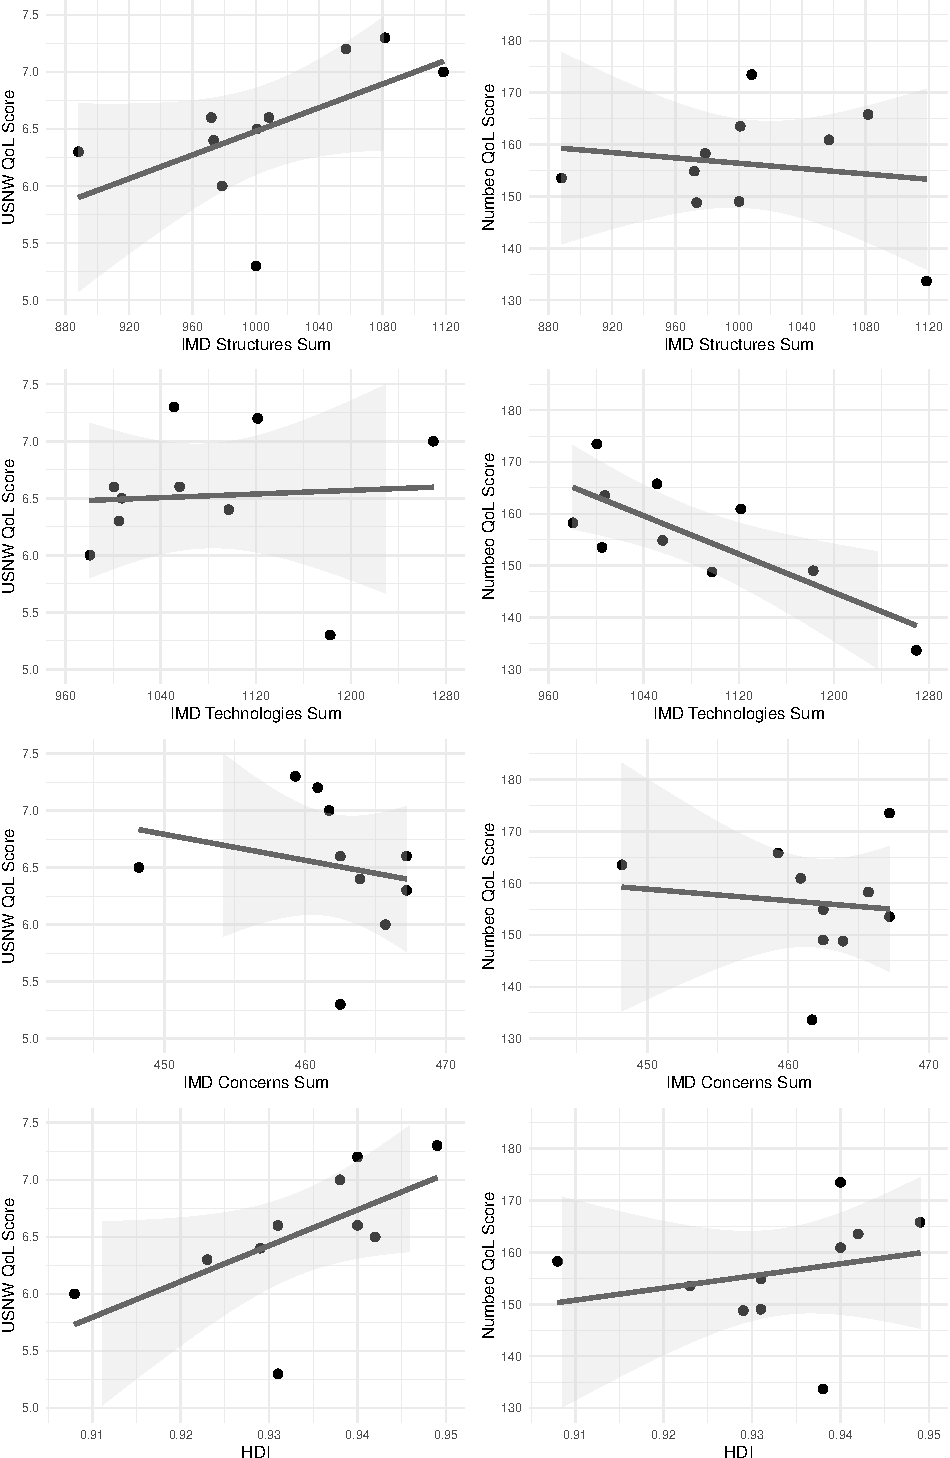
\includegraphics[keepaspectratio]{smartcities_files/figure-pdf/imddomainsvsqolplot-1.pdf}}

}

\caption{Associations between SCD domain scores, as evaluated by IMD,
and QoL scores}

\end{figure}%

As shown earlier, the sum of IMD Concerns indicators deviates
significantly from normality. Accordingly, correlations involving it
were assessed using Spearman's method, while the other IMD domains were
tested with Pearson's method.

Among USNW-related associations, a moderate positive correlation was
found with sum of IMD Structures (r = 0.57, p = 0.086) and with HDI (r =
0.62, p = 0.057), although neither reached statistical significance. The
correlation between USNW QoL and sum of IMD Technologies was near zero
(r = 0.06, p = 0.863), and the Spearman correlation with sum IMD
Concerns was weak (ρ = -0.53, p = 0.118). Correlation analysis between
the USNW QoL score and the various items listed under IMD Structures
reveals that the better-asociated items are not necessarily those that
we normally associate with SCD, especially within the US/NIST paradigm.
For example, the item that best predicts a good USNW QoL score is the
availability of bars and museums (Table 1).

\begin{longtable}[]{@{}lrr@{}}
\toprule\noalign{}
IMD Structures component & Pearson r & p-value \\
\midrule\noalign{}
\endhead
\bottomrule\noalign{}
\endlastfoot
Cultural activities (shows, bars, and museums) are satisfactory & 0.771
& 0.009 \\
Minorities feel welcome & 0.721 & 0.019 \\
Air pollution is not a problem & 0.721 & 0.019 \\
Green spaces are satisfactory & 0.587 & 0.074 \\
Lifelong learning opportunities are provided by local institutions &
0.538 & 0.108 \\
\end{longtable}

For Numbeo QoL, no meaningful correlations were observed with the sum of
IMD Structures (r = -0.15, p = 0.675), HDI (r = 0.25, p = 0.494), or sum
of IMD Concerns (ρ = -0.15, p = 0.674). A significant negative
correlation was found between Numbeo QoL and sum of IMD Technologies (r
= -0.77, p = 0.009). Moreover, a large number of items that fit the
NIST/US definition of SCD, listed under IMD Technologies, are,
unexpectedly, negatively correlated with Numbeo.co QoL scores.

\begin{longtable}[]{@{}lrr@{}}
\toprule\noalign{}
IMD Technology component & Pearson r & p-value \\
\midrule\noalign{}
\endhead
\bottomrule\noalign{}
\endlastfoot
CCTV cameras has made residents feel safer & -0.861 & 0.001 \\
Online services provided by the city has made it easier to start a new
business & -0.807 & 0.005 \\
Car-sharing Apps have reduced congestion & -0.799 & 0.006 \\
Free public wifi has improved access to city services & -0.754 &
0.012 \\
Online scheduling and ticket sales has made public transport easier to
use & -0.751 & 0.012 \\
The city provides information on traffic congestion through mobile
phones & -0.737 & 0.015 \\
Bicycle hiring has reduced congestion & -0.734 & 0.016 \\
Processing Identification Documents online has reduced waiting times &
-0.728 & 0.017 \\
Online public access to city finances has reduced corruption & -0.712 &
0.021 \\
Apps that direct you to an available parking space have reduced journey
time & -0.703 & 0.023 \\
An online platform where residents can propose ideas has improved city
life & -0.686 & 0.029 \\
Online reporting of city maintenance problems provides a speedy solution
& -0.676 & 0.032 \\
Online voting has increased participation & -0.628 & 0.052 \\
IT skills are taught well in schools & -0.624 & 0.054 \\
Online purchasing of tickets to shows and museums has made it easier to
attend & -0.600 & 0.067 \\
\end{longtable}

These findings suggest a domain-specific relationship between QoL
metrics and technological SCD dimensions, with technological dimensions
showing a strong, negative association, particularly when assessed
through Numbeo.

\subsection{Several subdomains of Numbeo.com QoL metric negatively
correlate with technology
SCD}\label{several-subdomains-of-numbeo.com-qol-metric-negatively-correlate-with-technology-scd}

Despite the unassuming lack of correlation with various other general
metrics, Numbeo.com QoL metrics are solidly, and paradoxically
negatively corelated with technology-related SCD policies, as measured
by the IMD. In this section, we attempt to find which of the eight
dimensions of Numbeo.com QoL assessment are more impactd by tchnology
SCD policies. General trends may be visualized in Fig. 7.

\begin{figure}[H]

{\centering \pandocbounded{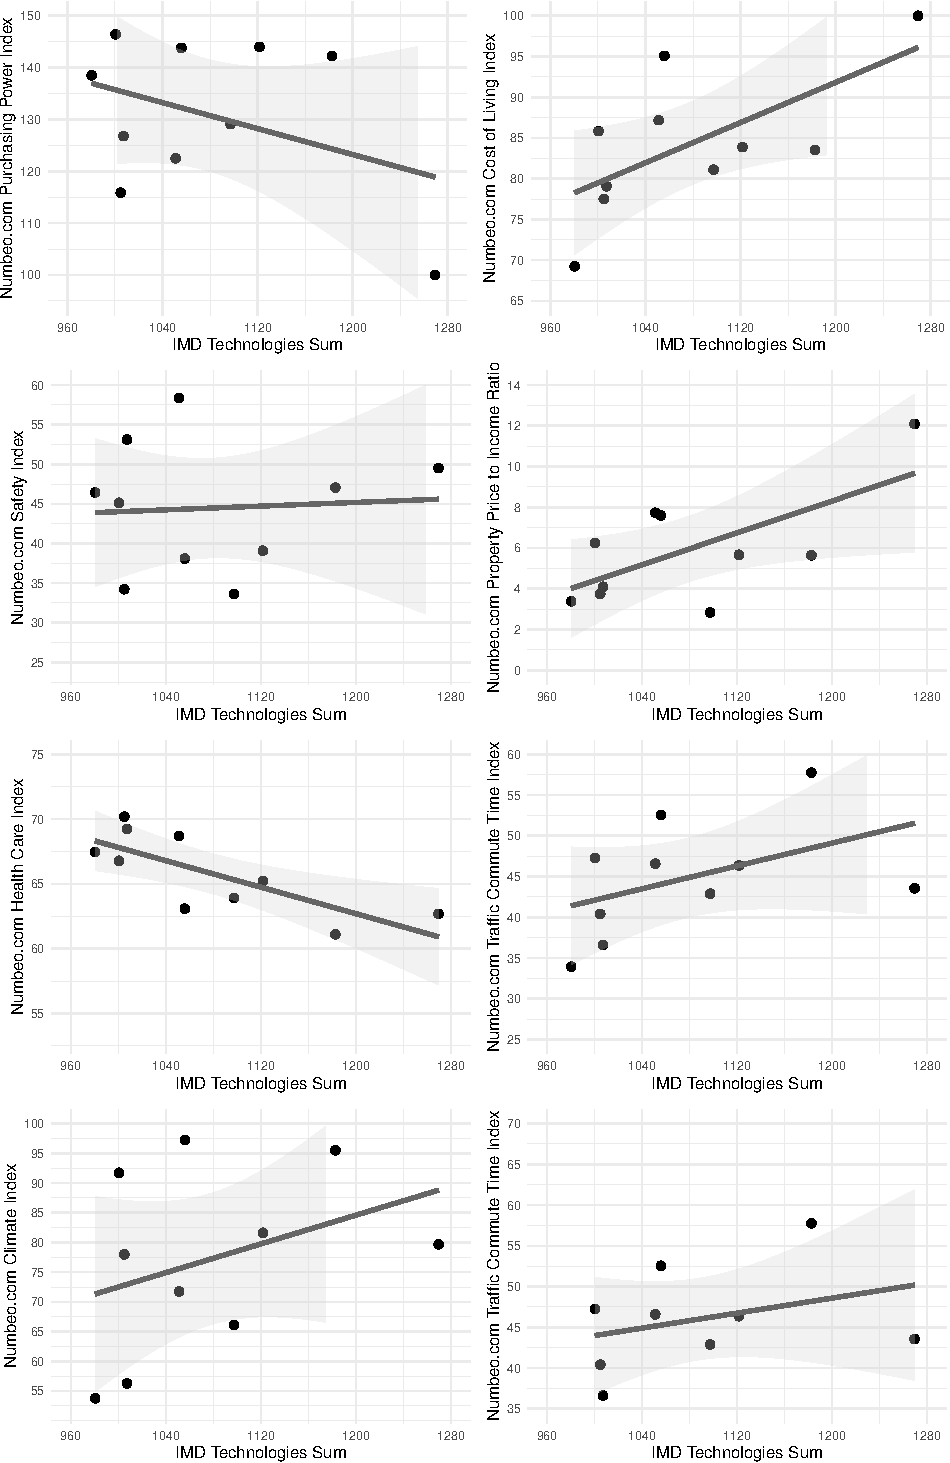
\includegraphics[keepaspectratio]{smartcities_files/figure-pdf/imdtechvsnumbeoplot-1.pdf}}

}

\caption{Associations between Numbeo.com QoL domain scores, as evaluated
by IMD, and sum of IMD Technologies indicators}

\end{figure}%

Normality of IMD Technologies Sum and all Numbeo component indices was
assessed using Shapiro-Wilk tests and was not rejected for any variable
(data not shown), justifying the use of Pearson correlations. Among the
eight Numbeo domains, three showed statistically significant
associations with IMD Technologies Sum: the Health Care Index (r =
-0.76, p = 0.01), the Cost of Living Index (r = 0.65, p = 0.04), and the
Property Price to Income Ratio (r = 0.66, p = 0.039). No other domain
displayed a significant correlation with IMD Technologies (data not
shown). In other words, Numbeo.com respondents rating QoL in high-tech
cities are negatively affected by increased cost of living, excessive
real estates prices by comparison with incomes, and reduced access to
quality healthcare.

\subsection{Multivariate linear regression models for the contribution
of various QoL components to the technology-associated
dissatisfaction}\label{multivariate-linear-regression-models-for-the-contribution-of-various-qol-components-to-the-technology-associated-dissatisfaction}

A multiple linear regression model was tested to predict IMD
Technologies Sum based on the three Numbeo dimensions shown earlier to
best correlate with it, namely Health Care Index, Property Price to
Income Ratio, and Cost of Living Index. The model showed a moderate fit
(adjusted R² = 0.608, p = NA). Among the predictors, only the Health
Care Index remained statistically significant (β = -19.38, p = 0.043),
while Property Price to Income Ratio (β = 20.5, p = 0.245) and Cost of
Living Index (β = -2.57, p = 0.656) were not. Residuals passed tests for
global normality (Jarque-Bera p = 0.502) and heteroskedasticity
(Breusch-Pagan p = 0.655). No autocorrelation was detected
(Durbin-Watson = 2.18, p = 0.7). However, Shapiro-Wilk test indicated
residual non-normality (p = 0.036), and multicollinearity analysis
revealed excessive inflation for Property Price to Income Ratio (VIF =
5.18) and Cost of Living Index (VIF = 6.12).

Given the lack of significance for the Cost of Living Index (p = 0.656)
and its substantial contribution to multicollinearity (VIF = 6.12), we
chose to drop this variable and pursue modling using the remaining two
predictors.

A second linear regression model was then estimated using only the
Health Care Index and Property Price to Income Ratio as predictors. The
model exhibited a strong fit (adjusted R² = 0.652, p = 0.01). The Health
Care Index was a statistically significant predictor (β = -17.84, p =
0.027), while Property Price to Income Ratio was marginally
non-significant (β = 13.95, p = 0.094). Multicollinearity diagnostics
confirmed acceptable VIF values for both predictors (VIF = 1.19 and 1.19
respectively). Residual analysis revealed no significant autocorrelation
(Durbin-Watson = 2.36, p = 0.678), no evidence of heteroskedasticity
(Breusch-Pagan p = 0.43), and satisfactory global normality of residuals
(Jarque-Bera p = 0.469). Additionally, the Shapiro-Wilk test for
residuals was non-significant (p = 0.089), confirming normality.

These results supported the selection of the two-predictor model as the
more robust specification. They provide strong support for a linear
relationship between improved IMD-evaluated SCD technologies and
perceived impaired access to quality healthcare, as reported by
Numbeo.com users. They also suggest a trend towards a second,
independent, QoL dimension being affected by SCD technologies, namely
housing costs.

\section{Discussion}\label{discussion}

In this study, we analyzed the correlations between smart city
development (SCD) metrics and quality of life (QoL) outcomes. Urban
development was assessed by two prestigious academic institutions, based
on scores derived from dozens of semi-independent elements, producing
rankings that have been republished for decades. The two SCD metrics
demonstrated a high degree of similarity. However, these metrics focus
on global rankings, generating very small samples. In contrast, QoL is a
well-established concept, which could have allowed for the inclusion of
a larger number of cities. Nonetheless, because QoL is a central theme
in political debates and cultural identity, no unique, standardized
definition exists, Unsurprisingly, the two QoL metrics used in this
study are not fully aligned.

A large part of the SCD metrics analyzed were not correlated with QoL
metrics. While in the case of the IESE metrics, such findings could be
attributed to smaller sample sizes, in the case of the IMD metrics we
described variable, occasionally very strong, correlations at domain-
and item-level with QoL metrics. Specifically, QoL as measured by USNW
criteria was positively correlated with the city-level estimated HDI and
with the IMD Structures indicator. The latter correlation could largely
be explained by the presence of green spaces and of theaters, museums,
and bars. By contrast, quality of life as estimated by USNW appeared to
be independent of the IMD Technologies index. The opposite situation was
observed for QoL life as estimated by the Numbeo algorithm. In this
case, the IMD Technologies index was the only SCD metric that correlated
with the QoL score. Surprisingly, the correlation was inverse (more
technology with poorer QoL), and could not be attributed to any specific
technological item. Two components among the eight included in the
Numbeo score --- namely, the quality of healthcare services and the
housing cost-to-income ratio --- largely explained this negative
correlation.

In conclusion, this study provides evidence that SCD can enhance QoL,
but also identifies contexts where this link does not translate into
perceived improvements for residents. Given the cross-sectional design,
no claims about temporal precedence or causality can be made.
Specifically, it appeears that SCD may primarily benefit younger,
healthier residents with discretionary income, while disadvantaging
renters and individuals with chronic illnesses.

A redefinition of urban development objectives, beyond current IESE and
IMD frameworks, may be necessary. For example, several indices used by
IESE are based on data from Numbeo. Since Numbeo captures perceived QoL
--- the outcome rather than the exposure --- it appears that the IESE
metrics reflect not just the development process, but tend to favor
local governments that succeed in achieving their targets, regardless of
the methods employed.

This study naturally has some limitations. First, most of the negative
results are likely to be type II errors, given the extremely small
sample size. However, expanding the sample to a significantly larger
volume is unlikely, as few municipalities possess the motivation,
vision, and funding necessary for effective SCD.

Another limitation is the lack of optimal data on QoL. Alternative
metrics exist, but they were not accessible during the drafting of this
analysis. Nevertheless, it should be noted that in most rankings, the
QoL situation tends to align more closely with what is reflected by
Numbeo, where New York City ranks well below Denver. Even the USNW
rankings have historically placed New York at a QoL level that is, at
best, mediocre compared to Denver, which is historically considered a
Top 10 city for QoL (Sparks
(\citeproc{ref-SparksNYCisnAmerica2019}{2019})).

During the research for this paper, we did not come across any
publication that applied quantitative methods to analyze the
relationship between SCD and QoL in the Western world. This gap may be
explained by the tautological nature of the subject, with the IESE and
IMD metrics serving as clear examples of confusion between mechanisms
and objectives. For instance, the number of museums may be seen more as
a goal --- a component of QoL --- rather than a lever for achieving the
goal, that is, a tool of SCD. Even so, this paper offers a good starting
point for critically evaluating what we currently call SCD, what opinion
leaders consider necessary for SCD progress, and what remains to be done
to achieve a more inclusive SCD.

\appendix

\section{Supplemental data}\label{supplemental-data}

\subsection{Supplemental Table 1. IMD Smart Cities Index 2023 components
(copied from Bris et al.,
2023)}\label{supplemental-table-1.-imd-smart-cities-index-2023-components-copied-from-bris-et-al.-2023}

Structures

\begin{itemize}
\tightlist
\item
  Healthcare and safety

  \begin{itemize}
  \tightlist
  \item
    Basic sanitation meets the needs of the poorest areas
  \item
    Recycling services are satisfactory
  \item
    Public safety is not a problem
  \item
    Air pollution is not a problem
  \item
    Medical services provision is satisfactory
  \item
    Finding housing with rent equal to 30\% or less of a monthly salary
    is not a problem
  \end{itemize}
\item
  Mobility

  \begin{itemize}
  \tightlist
  \item
    Traffic congestion is not a problem
  \item
    Public transport is satisfactory
  \end{itemize}
\item
  Leisure

  \begin{itemize}
  \tightlist
  \item
    Activități din timpul liber
  \item
    Green spaces are satisfactory
  \item
    Cultural activities (shows, bars, and museums) are satisfactory
  \end{itemize}
\item
  Professional devlopmet opporunities

  \begin{itemize}
  \tightlist
  \item
    Employment finding services are readily available
  \item
    Most children have access to a good school
  \item
    Lifelong learning opportunities are provided by local institutions
  \item
    Businesses are creating new jobs
  \item
    Minorities feel welcome
  \end{itemize}
\item
  Governance

  \begin{itemize}
  \tightlist
  \item
    Information on local government decisions are easily accessible
  \item
    Corruption of city officials is not an issue of concern
  \item
    Residents contribute to decision making of local government
  \item
    Residents provide feedback on local government project
  \end{itemize}
\end{itemize}

Technologies

\begin{itemize}
\tightlist
\item
  Healthcare and safety

  \begin{itemize}
  \tightlist
  \item
    Online reporting of city maintenance problems provides a speedy
    solution
  \item
    A website or App allows residents to easily give away unwanted items
  \item
    Free public wifi has improved access to city services
  \item
    CCTV cameras has made residents feel safer
  \item
    A website or App allows residents to effectively monitor air
    pollution
  \item
    Arranging medical appointments online has improved access
  \end{itemize}
\item
  Mobility

  \begin{itemize}
  \tightlist
  \item
    Car-sharing Apps have reduced congestion
  \item
    Apps that direct you to an available parking space have reduced
    journey time
  \item
    Bicycle hiring has reduced congestion
  \item
    Online scheduling and ticket sales has made public transport easier
    to use
  \item
    The city provides information on traffic congestion through mobile
    phones
  \end{itemize}
\item
  Leisure

  \begin{itemize}
  \tightlist
  \item
    Online purchasing of tickets to shows and museums has made it easier
    to attend
  \end{itemize}
\item
  Personal development opportunities

  \begin{itemize}
  \tightlist
  \item
    Online access to job listings has made it easier to find work
  \item
    IT skills are taught well in schools
  \item
    Online services provided by the city has made it easier to start a
    new business
  \item
    The current internet speed and reliability meet connectivity needs''
  \end{itemize}
\item
  Governance

  \begin{itemize}
  \tightlist
  \item
    Online public access to city finances has reduced corruption
  \item
    Online voting has increased participation
  \item
    An online platform where residents can propose ideas has improved
    city life
  \item
    Processing Identification Documents online has reduced waiting times
  \end{itemize}
\end{itemize}

Concerns:

\begin{itemize}
\tightlist
\item
  affordable housing
\item
  air pollution
\item
  basic amenities
\item
  citizen engagement
\item
  corruption
\item
  fulfilling employment
\item
  green spaces
\item
  health services
\item
  public transport
\item
  recycling
\item
  road congestion
\item
  school education
\item
  security
\item
  social mobility
\item
  unemployment.
\end{itemize}

\subsection{Supplemental Table 2. IESE Smart Cities 2024 components
(copied from Berrone et al.,
2024).}\label{supplemental-table-2.-iese-smart-cities-2024-components-copied-from-berrone-et-al.-2024.}

Human capital:

\begin{itemize}
\tightlist
\item
  Proportion of population with secondary and higher education
\item
  Number of public and private schools in the city
\item
  Number of business schools in the city included in the Financial Times
  TOP 100
\item
  Expenditure on education
\item
  Expenditure on leisure and recreation
\item
  Expenditure on leisure and recreation per capita
\item
  International flow of mobile students at the tertiary level
\item
  Number of museums and art galleries in the city
\item
  Number of TOP 500 universities
\item
  Number of theaters in the city
\end{itemize}

Social cohesion:

\begin{itemize}
\tightlist
\item
  Variable that indicates whether a city provides a friendly environment
  for women (on a scale of 1 to 5).
\item
  Number of public and private hospitals in the city
\item
  Estimation of the general level of crime in a city
\item
  Variable representing the national government's response to situations
  of slavery in the country.
\item
  Variable representing \ldots{} overall happiness
\item
  Gini Index
\item
  Index measuring the level of peace/violence in a country or region.
\item
  Estimation of the overall quality of the health care system, health
  care professionals, equipment, costs
\item
  Variable indicating whether a city provides a friendly environment for
  the LGBTQ+ community
\item
  Property price as a percentage of income.
\item
  Rate of female employment in the public sector.
\item
  Death rate per 100,000 city inhabitants.
\item
  Unemployment rate (number of unemployed/labor force).
\item
  Murder rate per 100,000 city inhabitants.
\item
  Suicide rate per 100,000 city inhabitants.
\item
  Number of terrorist incidents in the city in the last three years.
\item
  Index of racial tolerance in a city.
\end{itemize}

Economy:

\begin{itemize}
\tightlist
\item
  Number of unicorn companies in the city
\item
  Index \ldots{} higher for cities that have a more favorable regulatory
  environment for setting up and operating a local business.
\item
  Ranking of startup ecosystems.
\item
  Mortgage as a percentage of income is the monthly mortgage cost as a
  proportion of household income (the lower the better).
\item
  The percentage of opportunity-driven early-stage entrepreneurs divided
  by the percentage of necessity-driven early-stage entrepreneurs.
\item
  Number of headquarters of publicly traded companies.
\item
  Number of Fortune 500 companies present in the city.
\item
  Gross domestic product in millions of US dollars.
\item
  Projected growth in gross domestic product for the next year.
\item
  Gross domestic product per capita.
\item
  Purchasing power in buying goods and services in the city (based on
  the average salary), compared to that of New York City residents.
\item
  Labor productivity calculated as GDP/employed population (in
  thousands).
\item
  Hourly wage in the city in US dollars.
\item
  Number of calendar days needed to complete the procedures to legally
  operate a business.
\end{itemize}

Governance:

\begin{itemize}
\tightlist
\item
  Whether or not Bitcoin is legal in the city.
\item
  Whether or not the city has ISO 37120 certification. Certified cities
  are committed to improving urban services and quality of life.
\item
  Number of government buildings and premises in the city.
\item
  Number of embassies in the city.
\item
  Percentage of employed population working in public administration and
  defense; education; health; community, social and personal service
  activities; and other activities.
\item
  Index supplementing the E-Government Development Index (EGDI), which
  focuses on the use of online services to facilitate provision of
  information by governments to citizens (``e-information sharing''),
  interaction with stakeholders (``e-consultation''), and engagement in
  decision-making processes (``e-decision-making'').
\item
  Variable that reflects the human capacity dimension, which is one of
  the three dimensions that make up the EGDI (online service,
  telecommunication connectivity, and human capacity).
\item
  Index that measures the degree to which collateral and bankruptcy laws
  protect the rights of borrowers and lenders and thus facilitate access
  to loans.
\item
  Variable that reflects the development status of telecommunication
  infrastructure, which is one of the three dimensions that make up the
  EGDI (online service, telecommunication connectivity, and human
  capacity).
\item
  Corruption Perceptions Index
\item
  Variable that reflects the scope and quality of online services, which
  is one of the three dimensions that make up the EGDI (online service,
  telecommunication connectivity, and human capacity).
\item
  Number of research and technology offices in the city.
\item
  Whether or not the city has an open data system.
\item
  Democracy Index - The top-ranked countries are the ones considered
  most democratic.
\item
  Total reserves in millions of current dollars. City-level estimate
  based on population.
\item
  Reserves per capita in millions of current dollars.
\end{itemize}

Environment:

\begin{itemize}
\tightlist
\item
  Index of pollution.
\item
  Index of carbon dioxide emissions.
\item
  Carbon dioxide emissions from fossil fuel use and cement production.
\item
  Methane emissions caused by human activities such as agriculture and
  industrial methane production.
\item
  Environmental Performance Index
\item
  PM10, PM2.5 - air particulate pollutants
\item
  Percentage of the population with reasonable access to an appropriate
  quantity of water resulting from an improvement in the supply.
\item
  Renewable water resources per capita.
\item
  Average amount of municipal solid waste generated annually per person
  (kg/year).
\item
  Risk to the city due to climate change.
\end{itemize}

Mobility:

\begin{itemize}
\tightlist
\item
  Whether or not the city has a bicycle, moped or scooter rental
  service.
\item
  Number of shared bicycles in the city.
\item
  Number of metro stations in the city. Number of metro lines in the
  city. Length of the metro system in the city
\item
  Index estimating traffic inefficiencies.
\item
  Index of traffic and congestion in the city.
\item
  Index that is estimated by considering time spent in traffic. It is
  assumed that travel time dissatisfaction increases exponentially
  beyond 25 minutes.
\item
  Percentage of households with bicycles.
\item
  Variable that shows whether the city has a high-speed train or not.
\item
  Number of commercial vehicles in the city.
\item
  Number of inbound flights (air routes) in a city.
\end{itemize}

Urban planning:

\begin{itemize}
\tightlist
\item
  Number of bike-rental or bike-sharing points, based on docking
  stations where they can be picked up and dropped off.
\item
  Whether or not the city has a bike-sharing system.
\item
  The number of completed buildings in a city.
\item
  Electric car charging points in the city.
\item
  Percentage of the urban population that uses at least basic sanitation
  services---that is, improved sanitation facilities that are not shared
  with other households.
\item
  Whether or not the city has AI projects.
\item
  Percentage of buildings classified as high-rises. A high-rise is a
  multi-floored building of at least 12 stories or 35 m in height (115
  feet).
\item
  Number of deaths in traffic accidents per 100,000 inhabitants.
\end{itemize}

Intenational profile:

\begin{itemize}
\tightlist
\item
  Annual number of passengers per airport in thousands.
\item
  Number of hotels per capita.
\item
  The Restaurant Price Index compares the price of meals and drinks in
  restaurants and bars in a city to prices in New York City.
\item
  Number of McDonald's outlets in the city.
\item
  Number of international congresses and meetings held in a city.
\end{itemize}

Technology:

\begin{itemize}
\tightlist
\item
  Active mobile broadband subscriptions.
\item
  Innovation Cities Index
\item
  Percentage of households with Internet access.
\item
  Percentage of households with a personal computer.
\item
  Number of mobile phones per 100 inhabitants.
\item
  Registered X users in a city (in thousands of individuals) + number of
  registered LinkedIn members in the city.
\item
  Broadband subscriptions per 100 inhabitants.
\item
  Percentage of households with some kind of telephone service.
\item
  Fixed-line Internet speed in megabytes per second by country.
\item
  Mobile speed in megabytes per second (country).
\item
  Number of options for connecting to the Internet in a city.
\end{itemize}

\subsection{Supplemental Table 3. Components of USNW QoL Scores (copied
from How we rank the Best Places to Live and Retire, U.S. News \& World
Report, as of April
2024)}\label{supplemental-table-3.-components-of-usnw-qol-scores-copied-from-how-we-rank-the-best-places-to-live-and-retire-u.s.-news-world-report-as-of-april-2024}

\begin{itemize}
\tightlist
\item
  Crime Rate index (25\% of QoL score) is computed using murder, violent
  crime and property crime per-capita rates, from FBI's Uniform Crime
  Reports.
\item
  Quality of Education index (19\%) is computed using the average
  college readiness score from the US News Best High Schools rankings.
\item
  Well-being (index 19\%) use resident satisfaction scores regarding
  purpose, social, financial, community and physical We used the
  composite score, from Sharecare's Community Well-Being Index.
\item
  Commuter Index (16\%) uses time spent traveling door to door, whether
  by foot, public transit, car or bicycle, from US Census Bureau.
\item
  Quality and Availability of Health Care (9\%) uses the quantity of
  ranked facilities within 50, 100 and 250 miles of each metro area from
  US News Best Hospitals .
\item
  Air Quality Index (7\%) uses the homonymous index from the
  Environmental Protection Agency.
\item
  National Risk Index (5\%) uses risk to 18 types of natural hazards
  from Federal Emergency Management Agency, and community risk factors,
  including social vulnerability and community resilience.
\end{itemize}

\subsection{Supplemental Table 4. Numbero.com QoL score components
(paraphrased from numbeo.com, as of April
2024)}\label{supplemental-table-4.-numbero.com-qol-score-components-paraphrased-from-numbeo.com-as-of-april-2024}

The Cost of Living Index is a weighted mean of readers' submitted prices
for:

\begin{itemize}
\tightlist
\item
  Restaurants (such as McMeal at McDonalds, Meal at Inexpensive
  Restaurant, Meal at Mid-range Restaurant, Domestic Beer, Imported Beer
  and so on)
\item
  Food Markets
\item
  Transportation
\item
  Utilities
\item
  Sports And Leisure
\item
  Childcare
\item
  Clothing And Shoes.
\end{itemize}

The Purchasing Power Index is the ratio between:

\begin{itemize}
\tightlist
\item
  readers' submitted rents and Cost of Living prices (from the previous
  indicator)
\item
  readers' submitted net salaries.
\end{itemize}

The Property Price to Income Ratio (sometimes referred to as Housing
Affordability) estimates the number of years of family income required
to purchase a typical apartment outright, without a mortgage.

\begin{itemize}
\tightlist
\item
  Family income is calculated as 1.5 times the net salaries submitted by
  readers.
\item
  The typical apartment has 90 square meters, and is not located in
  downtown areas. Prices are submitted by readers.
\end{itemize}

The Safety Index (sometimes referred to by its inverse, Crime Index),
based on readers' responses about:

\begin{itemize}
\tightlist
\item
  General perception of crime levels
\item
  Perceived safety during daylight and nighttime
\item
  Concerns about specific crimes (mugging, robbery, car theft, physical
  attacks, public harassment, and bias-motivated incidents)
\item
  Property crime severity (burglary, theft, vandalism)
\item
  Violent crime severity (assault, homicide, sexual offenses).
\end{itemize}

The Healthcare Quality uses readers' responses about healthcare
providers, be they individuals or orgnizations, from the point of view
of:

\begin{itemize}
\tightlist
\item
  skill and competency
\item
  speed
\item
  modern equipment
\item
  accuracy and completeness
\item
  friendliness and courtesy
\item
  responsiveness waitings
\item
  location
\item
  cost.
\end{itemize}

The Climate Index is calculated from the temperature and dew point
(unspecifid source).

The Pollution Index is calculated from data, from World Health
Organization and from readers, about:

\begin{itemize}
\tightlist
\item
  Air and Water Pollution
\item
  Garbage Disposal and Cleanliness
\item
  Noise and Light Pollution
\item
  Availability of Green Spaces
\item
  Overall Pollution Comfort.
\end{itemize}

Traffic and Commute Times Index is calculated using reader's submitted
estimates for:

\begin{itemize}
\tightlist
\item
  overall traffic system inefficiencies
\item
  commute time
\item
  dissatisfaction with time spent in traffic
\item
  CO2 emissions (indirectly estimated from commute time).
\end{itemize}

\section*{References}\label{references}
\addcontentsline{toc}{section}{References}

\phantomsection\label{refs}
\begin{CSLReferences}{1}{0}
\bibitem[\citeproctext]{ref-BarrettInvestigateYouExpatriate2010}
Barrett, William P. 2010. {``Investigate {Before You Expatriate}.''}
June 10, 2010.
\url{https://www.forbes.com/forbes/2010/0628/investment-guide-retirement-medicare-taxes-investigate-before-expatriate.html}.

\bibitem[\citeproctext]{ref-Baudet-MichelChapitredecroissanceurbaine2021}
Baudet-Michel, Sophie, and Fabien Paulus. 2021. {``Chapitre 4. La
décroissance urbaine en France : mise en perspective par les recherches
sur les Shrinking Cities et les Systèmes urbains.''} In \emph{Déclin
urbain}, 129--62. Savoir/Agir. Vulaines-sur-Seine: Éditions du Croquant.
\url{https://doi.org/10.3917/asava.beal.2021.01.0129}.

\bibitem[\citeproctext]{ref-BerroneIESECitiesMotion2024}
Berrone, Pascual, Joan Enric Ricart, Federico Grossi, David Augusto
Giuliodori, and María Andrea Giuliodori. 2024. {``{IESE Cities} in
{Motion} 2024.''} IESE Business School - University of Navarra.
\url{https://www.iese.edu/media/research/pdfs/ST-0649-E}.

\bibitem[\citeproctext]{ref-BerroneIESECitiesMotion2014}
Berrone, Pascual, Joan Enric Ricart, Roger Ricart, Carlos Carrasco, Juan
Manuel Barrionuevo, David Augusto Giuliodori, Franco Boneu, and María
Andrea Giuliodori. 2014. {``{IESE Cities} in {Motion} 2014.''} IESE
Business School - University of Navarra.
\url{https://www.iese.edu/wp-content/uploads/2019/05/ST-0333.pdf?}

\bibitem[\citeproctext]{ref-BestPlacesLive2023}
{``Best {Places to Live} for Quality of Life, Ranked.''} 2023. U.S. News
\& World Report. November 6, 2023.
\url{https://realestate.usnews.com/places/rankings/best-places-to-live-for-quality-of-life}.

\bibitem[\citeproctext]{ref-Bloom25Citiesbest2024}
Bloom, Laura Begley. 2024. {``The 25 {U.S.} Cities with the Best Quality
of Life, Ranked in a New Report.''} \emph{Forbes}, February.
\url{https://www.forbes.com/sites/laurabegleybloom/2024/02/26/ranked-the-25-us-cities-with-the-best-quality-of-life-according-to-a-new-report/}.

\bibitem[\citeproctext]{ref-BolivarsearchSmartSource2019}
Bolívar, Manuel Pedro Rodríguez. 2019. {``In the Search for the
{`{Smart}'} {Source} of the Citizen's Perception of {Quality} of {Life}
in {European Smart Cities}.''} In \emph{Proceedings of the 52nd {Hawaii
International Conference} on {System Sciences}}.

\bibitem[\citeproctext]{ref-BrisIMDSmartCity2023}
Bris, Arturo, Christos Cabolis, Bruno Lanvin, Odete Madureira, José
Caballero, Marco Pistis, Maryam Zargari, and Alice Tozer. 2023. {``{IMD
Smart City Index Report} 2023.''}
\url{https://www.imd.org/wp-content/uploads/2023/04/smartcityindex-2023-v7.pdf?}

\bibitem[\citeproctext]{ref-CaragliuSmartcitiesEurope2011}
Caragliu, Andrea, Chiara Del Bo, and Peter Nijkamp. 2011. {``Smart
Cities in {Europe}.''} \emph{Journal of Urban Technology}, April.
\url{https://www.tandfonline.com/doi/abs/10.1080/10630732.2011.601117}.

\bibitem[\citeproctext]{ref-Choicomparativeanalysisseven2023}
Choi, Jeongbae, and Carlos E. Caicedo. 2023. {``A Comparative Analysis
of Seven {Smart City} Development Projects: {Institutional}, Economic,
Technical, and Policy Perspectives.''} In \emph{Proceedings of the 56th
{Hawaii International Conference} on {System Sciences}}.
\url{https://doi.org/10.24251/HICSS.2023.246}.

\bibitem[\citeproctext]{ref-EuropeanCommissionSmartcities2016}
European Commission. 2016. {``Smart Cities.''} 2016.
\url{https://commission.europa.eu/eu-regional-and-urban-development/topics/cities-and-urban-development/city-initiatives/smart-cities_en}.

\bibitem[\citeproctext]{ref-FreyNewcensusdata2024}
Frey, William H. 2024. {``New Census Data Hints at an Urban Population
Revival, Assisted by Immigration.''} Brookings. April 15, 2024.
\url{https://www.brookings.edu/articles/new-census-data-hints-at-an-urban-population-revival-assisted-by-immigration/}.

\bibitem[\citeproctext]{ref-Howwerank2024}
{``How We Rank the {Best Places to Live and Retire}.''} n.d. US News \&
World Report. Accessed April 25, 2024.
\url{https://realestate.usnews.com/places/methodology}.

\bibitem[\citeproctext]{ref-KugelThingsYouCan2016}
Kugel, Seth. 2016. {``8 Things You Can Do Now to Save Money on
Travel.''} \emph{The New York Times}, January 5, 2016.
\url{https://www.nytimes.com/2016/01/10/travel/cheap-airline-tickets-vacations.html}.

\bibitem[\citeproctext]{ref-LStaletwoecosystems2013}
L.S. 2013. {``A Tale of Two Ecosystems.''} \emph{The Economist}, October
3, 2013.
\url{https://www.economist.com/schumpeter/2013/10/03/a-tale-of-two-ecosystems}.

\bibitem[\citeproctext]{ref-MinisteriodeTransportesMovilidadyAgendaUrbanaDGdeViviendaySueloAreasurbanasEspana2022}
Ministerio de Transportes, Movilidad y Agenda Urbana, DG de Vivienda y
Suelo. 2022. {``Áreas urbanas en España 2022.''} November 2022.
\url{https://cvp.mitma.gob.es/downloadcustom/sample/3152}.

\bibitem[\citeproctext]{ref-MouratidisCompactcityurban2019}
Mouratidis, Kostas. 2019. {``Compact City, Urban Sprawl, and Subjective
Well-Being.''} \emph{Cities} 92 (September):261--72.
\url{https://doi.org/10/ghwg3x}.

\bibitem[\citeproctext]{ref-NationalRecordsofScotlandWebTeamPopulationGrowsLarge2021}
National Records of Scotland Web Team. 2021. {``Population {Grows} in
{Large Cities}, {Declines} in {Remote Areas}.''} Document. National
Records of Scotland. August 24, 2021.
\url{https://www.nrscotland.gov.uk/news/2021/population-grows-in-large-cities-declines-in-remote-areas}.

\bibitem[\citeproctext]{ref-NivolaAreEuropescities1999}
Nivola, Pietro S. 1999. {``Are {Europe}'s Cities Better?''} \emph{The
Public Interest} 137 (Autumn).
\url{https://www.brookings.edu/articles/are-europes-cities-better/}.

\bibitem[\citeproctext]{ref-Okulicz-KozarynEuropeansworklive2011}
Okulicz-Kozaryn, Adam. 2011. {``Europeans Work to Live and {Americans}
Live to Work ({Who} Is Happy to Work More: {Americans} or
{Europeans}?).''} \emph{Journal of Happiness Studies} 12 (2): 225--43.
\url{https://doi.org/10/djjmqh}.

\bibitem[\citeproctext]{ref-Okulicz-KozarynNourbanmalaise2019}
Okulicz-Kozaryn, Adam, and Rubia R. Valente. 2019. {``No Urban Malaise
for {Millennials}.''} \emph{Regional Studies}, February.
\url{https://www.tandfonline.com/doi/abs/10.1080/00343404.2018.1453130}.

\bibitem[\citeproctext]{ref-RCoreTeamlanguageenvironmentstatistical2021}
R Core Team. 2021. {``R: {A} Language and Environment for Statistical
Computing.''} R Foundation for Statistical Computing, Vienna, Austria.
2021. \url{http://www.r-project.org/index.html}.

\bibitem[\citeproctext]{ref-Samuelspollutedlifehighway2022}
Samuels, Gabe, and Yonah Freemark. 2022. {``The Polluted Life Near the
Highway. {A} Review of National Scholarship and a {Louisville} Case
Study.''} {Metropolitan Housing and Communities Policy Center}.
\url{https://www.urban.org/sites/default/files/2022-11/The\%20Polluted\%20Life\%20Near\%20the\%20Highway.pdf}.

\bibitem[\citeproctext]{ref-SerranoSmartcitiescommunities2022}
Serrano, Martin, Edward Griffor, David A. Wollman, Michael Dunaway,
Martin Burns, Sokwoo Rhee, and Chris Greer. 2022. {``Smart Cities and
Communities: {A} Key Performance Indicators Framework.''} \emph{NIST
Special Publication}, February.
\url{https://nvlpubs.nist.gov/nistpubs/SpecialPublications/NIST.SP.1900-206.pdf}.

\bibitem[\citeproctext]{ref-SparksNYCisnAmerica2019}
Sparks, Hannah. 2019. {``{NYC} Isn't {America}'s Best Place to Live --
and It's Not Even Close,''} April 10, 2019.
\url{https://nypost.com/2019/04/10/nyc-isnt-one-of-americas-best-places-to-live-and-its-not-even-close/}.

\bibitem[\citeproctext]{ref-StubingerUnderstandingSmartCity2020}
Stübinger, Johannes, and Lucas Schneider. 2020. {``Understanding {Smart
City} - {A} Data-Driven Literature Review.''} \emph{Sustainability} 12
(20): 8460. \url{https://doi.org/10/gjmz68}.

\bibitem[\citeproctext]{ref-UnitedNationsDepartmentofEconomicandSocialAffairsPopulationDivisionWorldCities20182018}
United Nations, Department of Economic and Social Affairs, Population
Division. 2018. {``The {World}'s Cities in 2018.''}
\url{https://www.un.org/development/desa/pd/sites/www.un.org.development.desa.pd/files/files/documents/2020/Jan/un_2018_worldcities_databooklet.pdf?}

\bibitem[\citeproctext]{ref-WangDoessmartcity2023}
Wang, Mengmeng, and Tao Zhou. 2023. {``Does Smart City Implementation
Improve the Subjective Quality of Life? {Evidence} from {China}.''}
\emph{Technology in Society} 72 (February):102161.
\url{https://doi.org/10/gtr4sj}.

\bibitem[\citeproctext]{ref-tidyverse2019}
Wickham, Hadley, Mara Averick, Jennifer Bryan, Winston Chang, Lucy
D'Agostino McGowan, Romain François, Garrett Grolemund, et al. 2019.
{``Welcome to the Tidyverse.''} \emph{Journal of Open Source Software} 4
(43): 1686. \url{https://doi.org/10.21105/joss.01686}.

\bibitem[\citeproctext]{ref-WintersUrbanisationnaturalamenities2016}
Winters, John V., and Yu Li. 2016. {``Urbanisation, Natural Amenities
and Subjective Well-Being: {Evidence} from {US} Counties.''} \emph{Urban
Studies}, February. \url{https://doi.org/10/gbj9nh}.

\end{CSLReferences}




\end{document}
